% Options for packages loaded elsewhere
\PassOptionsToPackage{unicode}{hyperref}
\PassOptionsToPackage{hyphens}{url}
\PassOptionsToPackage{dvipsnames,svgnames,x11names}{xcolor}
%
\documentclass[
]{article}

\usepackage{amsmath,amssymb}
\usepackage{iftex}
\ifPDFTeX
  \usepackage[T1]{fontenc}
  \usepackage[utf8]{inputenc}
  \usepackage{textcomp} % provide euro and other symbols
\else % if luatex or xetex
  \usepackage{unicode-math}
  \defaultfontfeatures{Scale=MatchLowercase}
  \defaultfontfeatures[\rmfamily]{Ligatures=TeX,Scale=1}
\fi
\usepackage{lmodern}
\ifPDFTeX\else  
    % xetex/luatex font selection
\fi
% Use upquote if available, for straight quotes in verbatim environments
\IfFileExists{upquote.sty}{\usepackage{upquote}}{}
\IfFileExists{microtype.sty}{% use microtype if available
  \usepackage[]{microtype}
  \UseMicrotypeSet[protrusion]{basicmath} % disable protrusion for tt fonts
}{}
\makeatletter
\@ifundefined{KOMAClassName}{% if non-KOMA class
  \IfFileExists{parskip.sty}{%
    \usepackage{parskip}
  }{% else
    \setlength{\parindent}{0pt}
    \setlength{\parskip}{6pt plus 2pt minus 1pt}}
}{% if KOMA class
  \KOMAoptions{parskip=half}}
\makeatother
\usepackage{xcolor}
\setlength{\emergencystretch}{3em} % prevent overfull lines
\setcounter{secnumdepth}{5}
% Make \paragraph and \subparagraph free-standing
\makeatletter
\ifx\paragraph\undefined\else
  \let\oldparagraph\paragraph
  \renewcommand{\paragraph}{
    \@ifstar
      \xxxParagraphStar
      \xxxParagraphNoStar
  }
  \newcommand{\xxxParagraphStar}[1]{\oldparagraph*{#1}\mbox{}}
  \newcommand{\xxxParagraphNoStar}[1]{\oldparagraph{#1}\mbox{}}
\fi
\ifx\subparagraph\undefined\else
  \let\oldsubparagraph\subparagraph
  \renewcommand{\subparagraph}{
    \@ifstar
      \xxxSubParagraphStar
      \xxxSubParagraphNoStar
  }
  \newcommand{\xxxSubParagraphStar}[1]{\oldsubparagraph*{#1}\mbox{}}
  \newcommand{\xxxSubParagraphNoStar}[1]{\oldsubparagraph{#1}\mbox{}}
\fi
\makeatother


\providecommand{\tightlist}{%
  \setlength{\itemsep}{0pt}\setlength{\parskip}{0pt}}\usepackage{longtable,booktabs,array}
\usepackage{calc} % for calculating minipage widths
% Correct order of tables after \paragraph or \subparagraph
\usepackage{etoolbox}
\makeatletter
\patchcmd\longtable{\par}{\if@noskipsec\mbox{}\fi\par}{}{}
\makeatother
% Allow footnotes in longtable head/foot
\IfFileExists{footnotehyper.sty}{\usepackage{footnotehyper}}{\usepackage{footnote}}
\makesavenoteenv{longtable}
\usepackage{graphicx}
\makeatletter
\newsavebox\pandoc@box
\newcommand*\pandocbounded[1]{% scales image to fit in text height/width
  \sbox\pandoc@box{#1}%
  \Gscale@div\@tempa{\textheight}{\dimexpr\ht\pandoc@box+\dp\pandoc@box\relax}%
  \Gscale@div\@tempb{\linewidth}{\wd\pandoc@box}%
  \ifdim\@tempb\p@<\@tempa\p@\let\@tempa\@tempb\fi% select the smaller of both
  \ifdim\@tempa\p@<\p@\scalebox{\@tempa}{\usebox\pandoc@box}%
  \else\usebox{\pandoc@box}%
  \fi%
}
% Set default figure placement to htbp
\def\fps@figure{htbp}
\makeatother
% definitions for citeproc citations
\NewDocumentCommand\citeproctext{}{}
\NewDocumentCommand\citeproc{mm}{%
  \begingroup\def\citeproctext{#2}\cite{#1}\endgroup}
\makeatletter
 % allow citations to break across lines
 \let\@cite@ofmt\@firstofone
 % avoid brackets around text for \cite:
 \def\@biblabel#1{}
 \def\@cite#1#2{{#1\if@tempswa , #2\fi}}
\makeatother
\newlength{\cslhangindent}
\setlength{\cslhangindent}{1.5em}
\newlength{\csllabelwidth}
\setlength{\csllabelwidth}{3em}
\newenvironment{CSLReferences}[2] % #1 hanging-indent, #2 entry-spacing
 {\begin{list}{}{%
  \setlength{\itemindent}{0pt}
  \setlength{\leftmargin}{0pt}
  \setlength{\parsep}{0pt}
  % turn on hanging indent if param 1 is 1
  \ifodd #1
   \setlength{\leftmargin}{\cslhangindent}
   \setlength{\itemindent}{-1\cslhangindent}
  \fi
  % set entry spacing
  \setlength{\itemsep}{#2\baselineskip}}}
 {\end{list}}
\usepackage{calc}
\newcommand{\CSLBlock}[1]{\hfill\break\parbox[t]{\linewidth}{\strut\ignorespaces#1\strut}}
\newcommand{\CSLLeftMargin}[1]{\parbox[t]{\csllabelwidth}{\strut#1\strut}}
\newcommand{\CSLRightInline}[1]{\parbox[t]{\linewidth - \csllabelwidth}{\strut#1\strut}}
\newcommand{\CSLIndent}[1]{\hspace{\cslhangindent}#1}

\usepackage[noblocks]{authblk}
\renewcommand*{\Authsep}{, }
\renewcommand*{\Authand}{ and }
\renewcommand*{\Authands}{, }
\renewcommand\Affilfont{\small}
\makeatletter
\@ifpackageloaded{tcolorbox}{}{\usepackage[skins,breakable]{tcolorbox}}
\@ifpackageloaded{fontawesome5}{}{\usepackage{fontawesome5}}
\definecolor{quarto-callout-color}{HTML}{909090}
\definecolor{quarto-callout-note-color}{HTML}{0758E5}
\definecolor{quarto-callout-important-color}{HTML}{CC1914}
\definecolor{quarto-callout-warning-color}{HTML}{EB9113}
\definecolor{quarto-callout-tip-color}{HTML}{00A047}
\definecolor{quarto-callout-caution-color}{HTML}{FC5300}
\definecolor{quarto-callout-color-frame}{HTML}{acacac}
\definecolor{quarto-callout-note-color-frame}{HTML}{4582ec}
\definecolor{quarto-callout-important-color-frame}{HTML}{d9534f}
\definecolor{quarto-callout-warning-color-frame}{HTML}{f0ad4e}
\definecolor{quarto-callout-tip-color-frame}{HTML}{02b875}
\definecolor{quarto-callout-caution-color-frame}{HTML}{fd7e14}
\makeatother
\makeatletter
\@ifpackageloaded{caption}{}{\usepackage{caption}}
\AtBeginDocument{%
\ifdefined\contentsname
  \renewcommand*\contentsname{Table of contents}
\else
  \newcommand\contentsname{Table of contents}
\fi
\ifdefined\listfigurename
  \renewcommand*\listfigurename{List of Figures}
\else
  \newcommand\listfigurename{List of Figures}
\fi
\ifdefined\listtablename
  \renewcommand*\listtablename{List of Tables}
\else
  \newcommand\listtablename{List of Tables}
\fi
\ifdefined\figurename
  \renewcommand*\figurename{Figure}
\else
  \newcommand\figurename{Figure}
\fi
\ifdefined\tablename
  \renewcommand*\tablename{Table}
\else
  \newcommand\tablename{Table}
\fi
}
\@ifpackageloaded{float}{}{\usepackage{float}}
\floatstyle{ruled}
\@ifundefined{c@chapter}{\newfloat{codelisting}{h}{lop}}{\newfloat{codelisting}{h}{lop}[chapter]}
\floatname{codelisting}{Listing}
\newcommand*\listoflistings{\listof{codelisting}{List of Listings}}
\makeatother
\makeatletter
\makeatother
\makeatletter
\@ifpackageloaded{caption}{}{\usepackage{caption}}
\@ifpackageloaded{subcaption}{}{\usepackage{subcaption}}
\makeatother

\usepackage{bookmark}

\IfFileExists{xurl.sty}{\usepackage{xurl}}{} % add URL line breaks if available
\urlstyle{same} % disable monospaced font for URLs
\hypersetup{
  pdftitle={The Tethys Metadata Interface in PAMGuard},
  pdfauthor={Douglas Gillespie; Marie Roch},
  colorlinks=true,
  linkcolor={blue},
  filecolor={Maroon},
  citecolor={Blue},
  urlcolor={Blue},
  pdfcreator={LaTeX via pandoc}}


\title{The Tethys Metadata Interface in PAMGuard}


\author[1]{Douglas Gillespie}
\author[2]{Marie Roch}

\affil[1]{Sea Mammal Research Unit, University of St Andrews}
\affil[2]{San Diego State University, CA}


\date{2024-12-18}
\begin{document}
\maketitle

\section{Summary}
In this tutorial, you'll learn how to export data from \href{https://www.pamguard.org}{PAMGuard}  to a \href{https://tethys.sdsu.edu}{Tethys database}  and to view the exported data both within PAMGuard and through the Tethys web interface.

\href{https://tethys.sdsu.edu}{Tethys} is a temporal-spatial database for metadata related to passive     acoustic studies. Unlike the PAMGuard databases, which hold a lot of detail about a single dataset, a Tethys database can hold summary data for many projects -- that can be every project for you as an individual, your lab, or for multiple labs across a larger organisation.

Tethys does not replace existing PAMGuard databases and binary storage system since it's not possible to get the level of detail PAMGuard uses during analysis into a single general database. However, the intent is that Tethys will contain enough detail for extensive meta-analysis across large temporal and spatial scales, eliminating (or at least minimising) the requirement for researchers to go back to the original PAMGuard data sets.

\textbf{Learning Outcomes}
In this tutorial you wil learn to:
\begin{enumerate}
\item Install Tethys and launch the Tethys Server
\item Add a Tethys module to PAMGuard and connect to the Tethys Server
\item Export data from PAMGuard to Tethys, including:
\begin{itemize}
\item Calibration data
\item Deployment data
\item Detections
\end{itemize}
\item View the exported data from within PAMGuard and using the Tethys Web client
\end{enumerate}
\newpage

\renewcommand*\contentsname{Table of contents}
{
\hypersetup{linkcolor=}
\setcounter{tocdepth}{3}
\tableofcontents
}

\section{Introduction}\label{introduction}

In this tutorial, you'll learn how to export data from PAMGuard to a
Tethys database and to view the exported data both within PAMGuard and
through the Tethys web interface.

\href{https://tethys.sdsu.edu}{Tethys} is a temporal-spatial database
for metadata related to passive acoustic studies. Unlike the PAMGuard
databases, which hold a lot of detail about a single dataset, a Tethys
database can hold summary data for many projects -- that can be every
project for you as an individual, your lab, or for multiple labs across
a larger organisation.

Tethys does not replace existing PAMGuard databases and binary storage
system since it's not possible to get the level of detail PAMGuard uses
during analysis into a single general database. However, the intent is
that Tethys will contain enough detail for extensive meta-analysis
across large temporal and spatial scales, eliminating (or at least
minimising) the requirement for researchers to go back to the original
PAMGuard data sets.

\newpage{}

\section{Glossary}\label{glossary}

\begin{longtable}[]{@{}
  >{\raggedright\arraybackslash}p{(\linewidth - 2\tabcolsep) * \real{0.3425}}
  >{\raggedright\arraybackslash}p{(\linewidth - 2\tabcolsep) * \real{0.6575}}@{}}
\caption{Glossary of terms used in this
tutorial}\label{tbl-glossary}\tabularnewline
\toprule\noalign{}
\begin{minipage}[b]{\linewidth}\raggedright
Term
\end{minipage} & \begin{minipage}[b]{\linewidth}\raggedright
Meaning
\end{minipage} \\
\midrule\noalign{}
\endfirsthead
\toprule\noalign{}
\begin{minipage}[b]{\linewidth}\raggedright
Term
\end{minipage} & \begin{minipage}[b]{\linewidth}\raggedright
Meaning
\end{minipage} \\
\midrule\noalign{}
\endhead
\bottomrule\noalign{}
\endlastfoot
Tethys & Mother of the Greek river gods. (Also the name of a database
system designed to handle metadata from passive acoustic studies). \\
Tethys Server & Software that you'll run on your computer which controls
the database and allows other software to communicate with the database,
writing and reading records. \\
Tethys Database & A set of Tethys data records \\
Tethys Client & Software that can communicate with the Tethys Server.
The two clients you'll use in this tutorial are the Tethys Web client,
which runs in a web browser (Chrome, Firefox, etc.) and PAMGuard, though
you can also use Matlab, R, and other programming languages to build
your own Tethys clients. \\
PAMGuard & The PAMGuard software, containing a suite of detectors,
classifiers and localisers for different sound types. \\
PAMGuard dataset & Data output from PAMGuard. This generally comprises
both a PAMGuard database AND a PAMGuard binary store. A PAMGuard dataset
has information from a single device, usually from a single cruise.
e.g.~if you've been doing surveys from a single vessel over a period or
weeks or months, that should generate a single dataset. However, if
you'd deployed multiple autonomous recorders, or had two or more vessels
out working at the same time, you'd have multiple PAMGuard datasets. \\
PAMGuard database & One of the data storage systems PAMGuard uses. This
is a relational database (usually sqlite) containing information about
PAMGuard operation, configuration, and DCL output. \\
PAMGuard binary store & A set of bespoke data files associated with a
PAMGuard dataset. These can contain a lot more detail than the PAMGuard
database, provide more rapid data access times, etc. \\
\end{longtable}

\section{Installation}\label{installation}

You can carry out these exercises with any data you like, so long as you
have it set up for looking at in the PAMGuard Viewer. We've provided a
North Atlantic Right Whale dataset to get you going and the exercises
will refer specifically to detectors and operations possible with this
dataset. We recommend that you go through the exercises once with our
data, then go through them again with your own.

\subsection{Software}\label{software}

\subsubsection{PAMGuard}\label{pamguard}

This tutorial will work with
\href{https://www.pamguard.org/downloadsurvey.html}{PAMGuard version
2.02.14 or later}, and \href{https://zenodo.org/records/13626338}{Tethys
version 3.1}.

If you are running PAMGuard vesion 2.02.15 or earlier, you must enable
Tethys in PAMGuard by specifyng the -smru option as a command line
option (Figure~\ref{fig-smru}).

\begin{figure}

\centering{

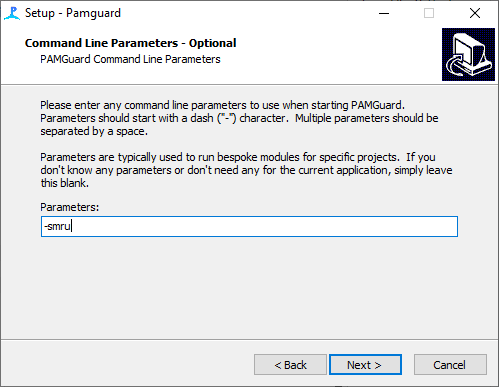
\includegraphics[width=11cm,height=\textheight,keepaspectratio]{./media/smruoption.png}

}

\caption{\label{fig-smru}Setting the command line option during
installation}

\end{figure}%

\subsubsection{Tethys}\label{tethys}

Download \href{https://zenodo.org/records/13626338}{Tethys 3.1 from
Zenodo}

\textbf{Marie - do you want to write instruction on starting Tethys or
provide your preferred link to instructions}

\subsubsection{SQLite Studio}\label{sqlite-studio}

It is not essential to download SQLite Studio, but if you want to easily
look inside the PAMGuard database you can
\href{https://sqlitestudio.pl/}{download it here}. Other viewers are
available, but this is the one we mostly use.

\subsection{Data}\label{data}

The dataset we'll be working with initially is seven days of right whale
data collected in Cape Cod Bay in 2008 with a Cornell MARU device. These
data were prepared for the 2013 DCLDE workshop held in St Andrews. To
save time, the data have already been processed using two different
right whale detectors: The Deep Learning detector
(\citeproc{ref-shiu2020}{Shiu et al. 2020}) and the older right whale
edge detector (\citeproc{ref-gillespie2004}{Gillespie 2004}). We've also
runsome noise measurements on the data. Output from the detectors is in
both the
\href{https://www.pamguard.org/olhelp/utilities/generalDatabaseHelp/docs/database_database.html}{PAMGuard
database} and set of
\href{https://www.pamguard.org/olhelp/utilities/BinaryStore/docs/binarystore_overview.html}{binary
files} which you can download the data here. Unzip the files into a
folder of your choice.

Having the wav files is not essential for the completion of the
exercises, but it's good to have them, or at least to know where they
are. Wav files are available as part of the
\href{https://doi.org/10.17630/62c3eebc-5574-4ec0-bfef-367ad839fe1a}{DCLDE
2013 workshop dataset}. You will need the zipped archive
\href{https://research-portal.st-andrews.ac.uk/files/264470819/NOPPWavFiles.zip}{NOPPWavFiles.zip}.
Download the files into a folder of your choice.

\section{Launch PAMGuard Viewer}\label{launch-pamguard-viewer}

The PAMGuard Tethys module is only available in
\href{https://www.pamguard.org/olhelp/overview/PamMasterHelp/docs/viewerMode.html}{Viewer
Mode}.

To get started, launch PAMGuard viewer mode, when it asks for a
database, navigate to the NARWExample.sqlite3 database that you
downloaded. When you launch the viewer, it will ask for the location of
the PAMGuard database (Figure~\ref{fig-launch}) and the PAMGuard binary
store (Figure~\ref{fig-binaryselect}). By default, it will probably look
for these files where I had them stored on my computer and you'll have
them somewhere else, so navigate carefully to the correct database file
and binary store.

\begin{figure}

\centering{

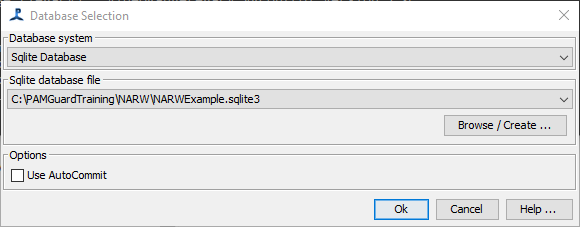
\includegraphics[width=0.7\linewidth,height=\textheight,keepaspectratio]{./media/launch.png}

}

\caption{\label{fig-launch}PAMGuard Viewer database selection}

\end{figure}%

\begin{figure}

\centering{

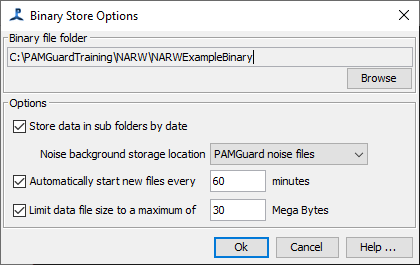
\includegraphics[width=0.7\linewidth,height=\textheight,keepaspectratio]{./media/binaryselect.png}

}

\caption{\label{fig-binaryselect}Selecting the binary storage location}

\end{figure}%

When asked for the binary file folder, navigate to where you stored the
binary file data you downloaded and select that folder:

Did you know that if you right click on the database file, you'll get an
option to open the database in the PAMGuard Viewer from Windows Explorer
(Figure~\ref{fig-dbmenu}).

\begin{figure}

\centering{

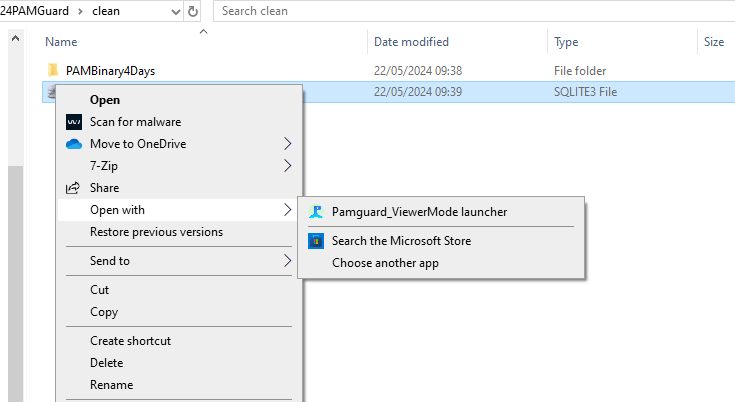
\includegraphics[width=0.7\linewidth,height=\textheight,keepaspectratio]{./media/dbmenuitem.png}

}

\caption{\label{fig-dbmenu}Menu Command to open the database}

\end{figure}%

If you've downloaded the raw recording files, you can tell PAMGuard
where to find these from the Settings / Sound Acquisition menu
(Figure~\ref{fig-wavfiles}). Note that having the raw audio available at
this point isn't essential.

\begin{figure}

\centering{

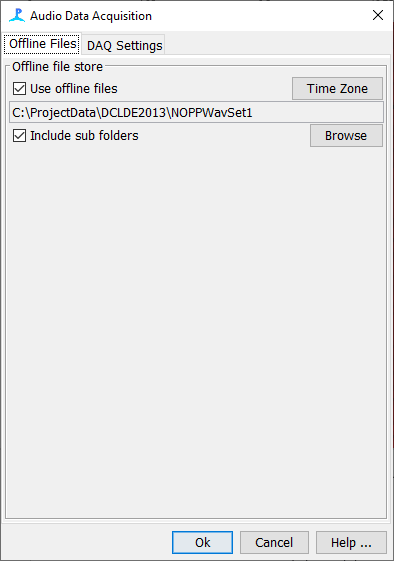
\includegraphics[width=0.6\linewidth,height=\textheight,keepaspectratio]{./media/wavfiles.png}

}

\caption{\label{fig-wavfiles}Setting the sound file location}

\end{figure}%

Have a quick scroll through the data and you should be able to see both
the DL detections, which appear as a shaded rectangle over the full
bandwidth of the spectrogram (Figure~\ref{fig-spectrogram}), and the
edge detections which show the outlines of the sounds. You'll probably
notice that there are more DL detections than there are edge detections.
This is because the DL detector is better than the edge detector as
shown in (\citeproc{ref-shiu2020}{Shiu et al. 2020}).

\begin{figure}

\centering{

\pandocbounded{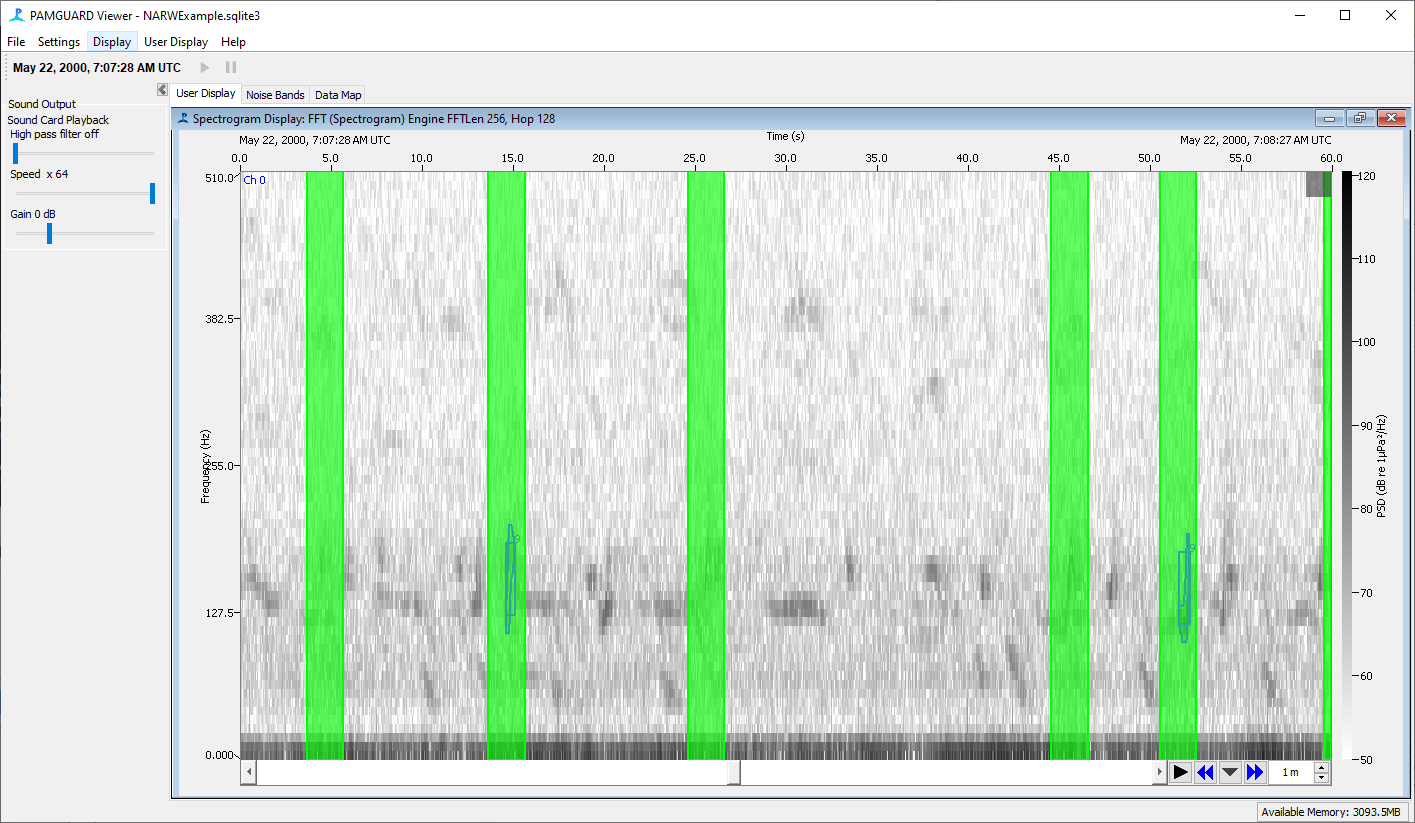
\includegraphics[keepaspectratio]{./media/spectrogram.png}}

}

\caption{\label{fig-spectrogram}Viewing data in the PAMGuard
spectrogram. The green bands are detections from the Deep LEarning
detector. The smaller marks are from the Right Whale Edge Detector}

\end{figure}%

\section{Add the Tethys Module}\label{add-the-tethys-module}

To communicate with Tethys, you'll first have to add the PAMGuard Tethys
module. This is available in the File / Add Modules / Utilities menu. If
you can't find it, then you've an old version of PAMGuard and not the
one we need, or you've not followed the PAMGuard installation
instructions properly and set the -smru option
((\citeproc{ref-fig}{\textbf{fig?}})--smru).

First time you run you may get a security warning
(Figure~\ref{fig-firewall}). Say OK to everything. If you don't have
admin rights, you may have difficulties here !

\begin{figure}

\centering{

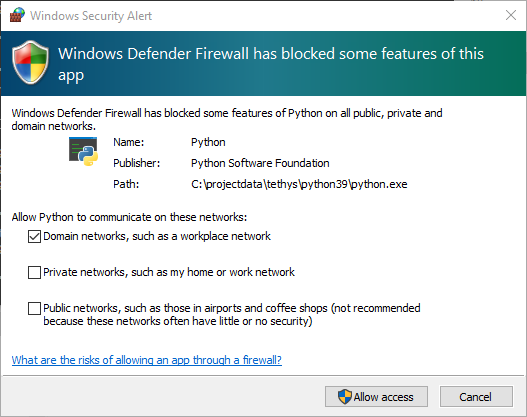
\includegraphics[width=0.7\linewidth,height=\textheight,keepaspectratio]{./media/firewall.png}

}

\caption{\label{fig-firewall}Windows security warning you'll get the
first time you run Tethys}

\end{figure}%

Once the Tethys module is added, go to the Tethys tab, the PAMGuard
display should look like (Figure~\ref{fig-tethys1}).

\begin{figure}

\centering{

\pandocbounded{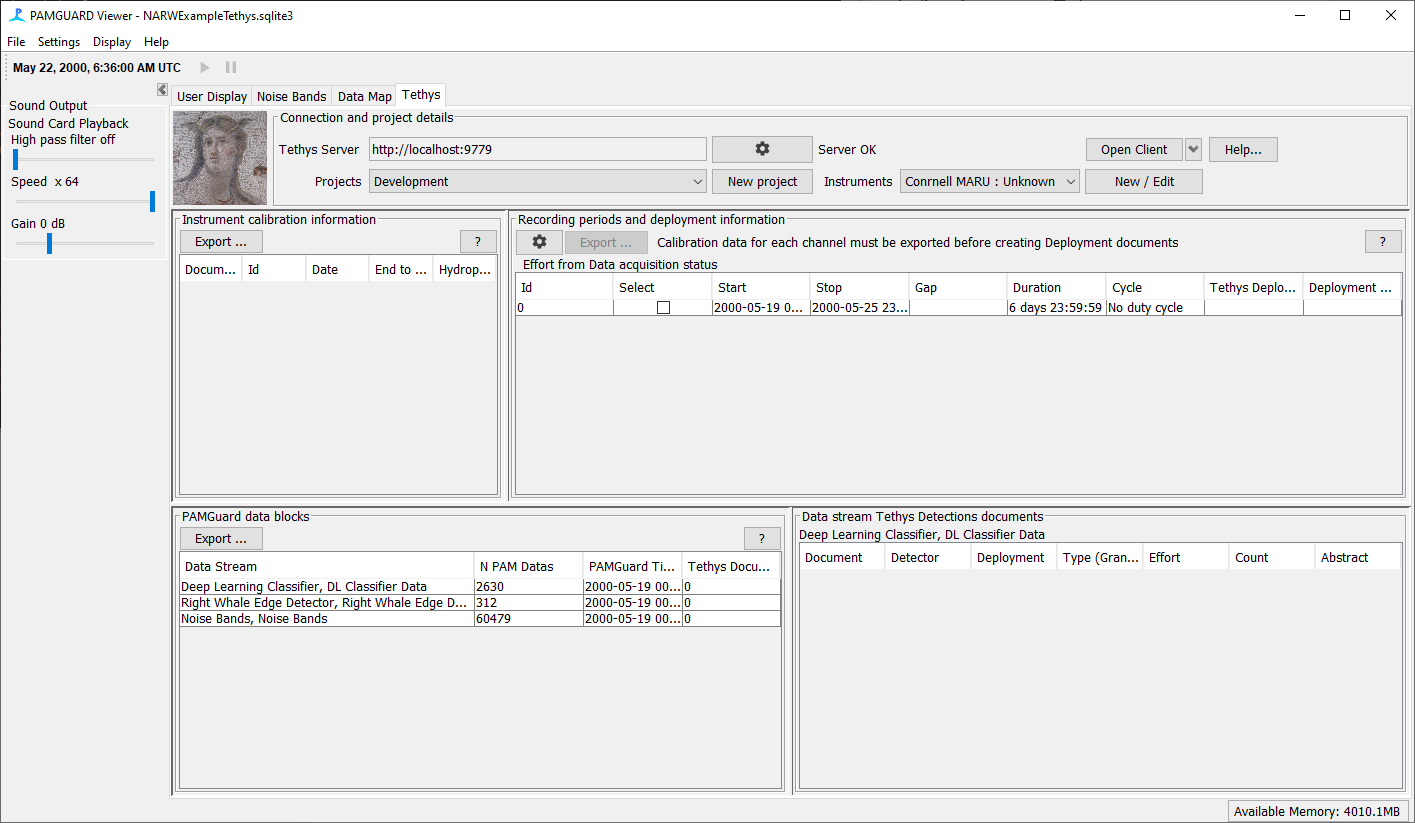
\includegraphics[keepaspectratio]{./media/tethys1.png}}

}

\caption{\label{fig-tethys1}The Tethys tab panel, currently showing an
error since the Tethys server has not yet been started}

\end{figure}%

If the top area of the display is coloured orange
(Figure~\ref{fig-tethys1}), then it means the Tethys server is not
running properly or that PAMGuard is failing to communicate with it.
Start the server according to the instructions in the installation
document. Once the server is running, the PAMGuard display will be a
normal grey colour. If you can't get this to work, ask for help!

\subsection{Project Information}\label{project-information}

A key goal of Tethys is accurate recording of project metadata. This
includes obvious information such as hydrophone calibrations and
locations of data, but also includes more nuanced information such as
the motivation for the project deployment and who the responsible person
for the data is. Additional project information data has been added to
PAMGuard in support of Tethys integration and should now be filled in.
This information is available in the Settings / Project Information
menu, or can be filled out as you export data to Tethys.

The project information follows the schema laid out in
(\citeproc{ref-roch2016}{Roch et al. 2016}) and you are encouraged to
fill in as much as possible. Since this is just a test, fill the data as
shown in Figure~\ref{fig-projectinfo}. Note that it's worth filling in
the project metadata for all PAMGuard projects, even if you don't use
Tethys. Do it at the start of your project while it's still fresh in
your mind.

\begin{figure}

\begin{minipage}{0.50\linewidth}

\centering{

\pandocbounded{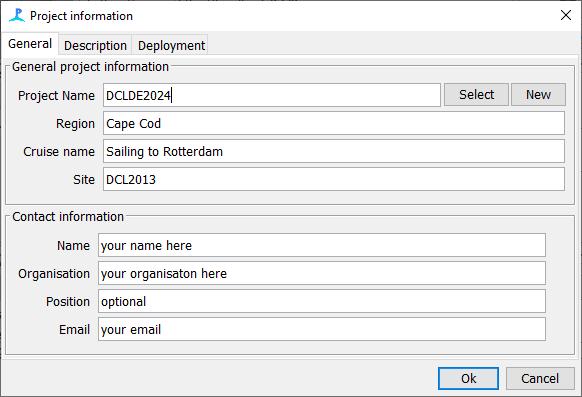
\includegraphics[keepaspectratio]{./media/project.png}}

}

\subcaption{\label{fig-project}General information}

\end{minipage}%
%
\begin{minipage}{0.50\linewidth}

\centering{

\pandocbounded{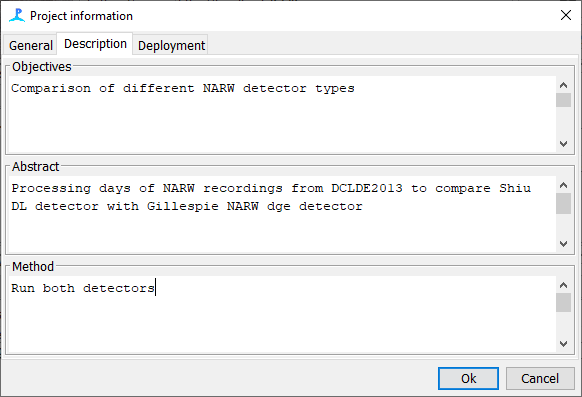
\includegraphics[keepaspectratio]{./media/projdescription.png}}

}

\subcaption{\label{fig-projdescription}Project description}

\end{minipage}%

\caption{\label{fig-projectinfo}PAMGuard dialog for project
information.}

\end{figure}%

In the `Deployment' tab, set it to ``Use start and end times of
collected audio data''

Obviously, for `real' data, you'd enter a lot more detail at this point.

\begin{tcolorbox}[enhanced jigsaw, titlerule=0mm, rightrule=.15mm, opacitybacktitle=0.6, breakable, colframe=quarto-callout-tip-color-frame, coltitle=black, toptitle=1mm, bottomtitle=1mm, colback=white, title=\textcolor{quarto-callout-tip-color}{\faLightbulb}\hspace{0.5em}{No promises, but there is no harm in asking \ldots{}}, arc=.35mm, bottomrule=.15mm, left=2mm, leftrule=.75mm, toprule=.15mm, colbacktitle=quarto-callout-tip-color!10!white, opacityback=0]

At this point in the software development, it's a really good time to
make suggestions. Do you want the boxes for project information to be
bigger ? How much text do you want to put into them ? Should you be
copying in your entire cruise research protocol ?

\end{tcolorbox}

\subsection{Hydrophone / Instrument
information}\label{hydrophone-instrument-information}

The hydrophone calibration and location information have already been
set in the PAMGuard database, but the discerning among you may notice
the additional ``Instrument Type'' and ``Instrument Id'' fields in the
hydrophone array configuration (Figure~\ref{fig-array}). These are
required by Tethys and, along with the project name, are used to link
Tethys data to PAMGuard data whenever the PAMGuard configuration is
opened with the Tethys database module in the future. These are part of
PAMGuard whether you use Tethys or not, and you're encouraged to fill
them to keep a record of what you've been doing.

\begin{figure}

\centering{

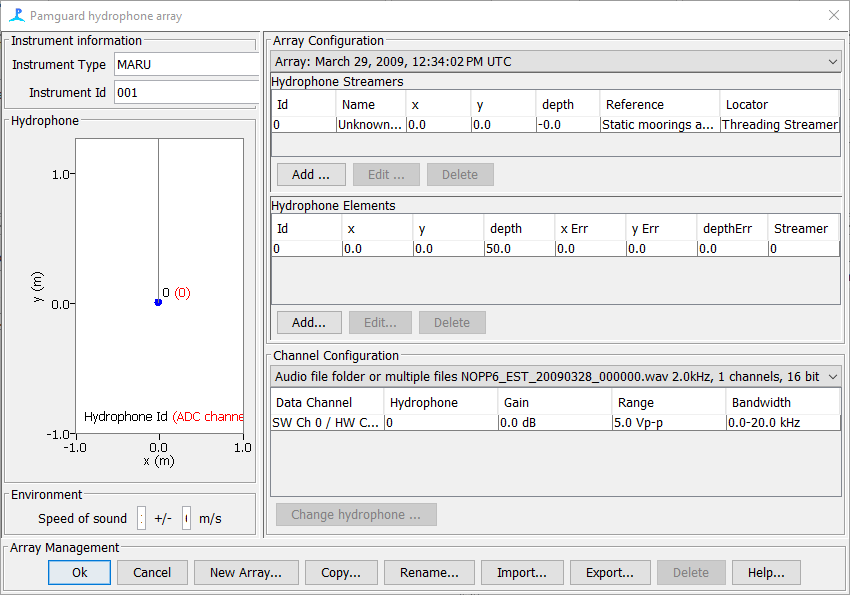
\includegraphics[width=0.8\linewidth,height=\textheight,keepaspectratio]{./media/arraymanager.png}

}

\caption{\label{fig-array}A screenshot of a computer Description
automatically generated}

\end{figure}%

\section{Tethys Data Export}\label{tethys-data-export}

There are four main types of Tethys document:

\textbf{Calibrations} -- information about the individual hydrophones
used.

\textbf{Deployments} -- information about deployment locations, dates,
motivations, etc.

\textbf{Detections} -- detections (or noise measurements) found within
the data.

\textbf{Localizations} -- localisations of detected sounds in one, two
or three dimensions.

These should be exported in order so that the Deployments can reference
the Calibrations and the Detections can reference the Deployments, etc.

\begin{tcolorbox}[enhanced jigsaw, titlerule=0mm, rightrule=.15mm, opacitybacktitle=0.6, breakable, colframe=quarto-callout-tip-color-frame, coltitle=black, toptitle=1mm, bottomtitle=1mm, colback=white, title=\textcolor{quarto-callout-tip-color}{\faLightbulb}\hspace{0.5em}{No promises, but there is no harm in asking \ldots{}}, arc=.35mm, bottomrule=.15mm, left=2mm, leftrule=.75mm, toprule=.15mm, colbacktitle=quarto-callout-tip-color!10!white, opacityback=0]

What types of calibration data do you have for your own studies ? Will
it fit into these data fields or do you require something different ?

\end{tcolorbox}

For each type of data, there is an export Wizard. Ideally, you should
know what to put in most of the data fields, but if you're exporting
older data may not be able to do this fully -- for example, we've no
idea how the data we're using in this example were calibrated, let alone
the serial number of the device used in the calibration. (Hopefully, the
data owners do know that, but we've not had time to dig that information
out). Going forwards, these are all things you should be noting down for
every one of your projects if you want the data to be useful in years to
come.

\subsection{Export the Calibrations}\label{export-the-calibrations}

(in this case there is only one hydrophone, so it's a `calibration')
fill in as much information as you can in the dialog panels
(Figure~\ref{fig-cal}). You'll get either a popup windows telling you
that the export has succeeded, or an error message.

\begin{figure}

\begin{minipage}{0.50\linewidth}

\centering{

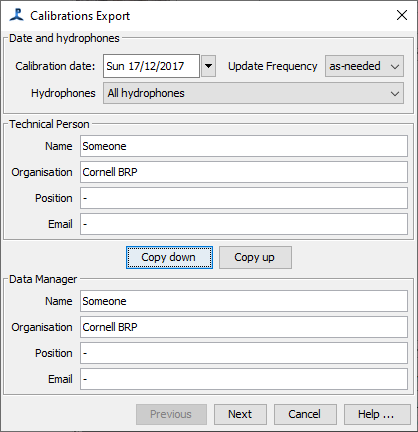
\includegraphics[width=0.98\linewidth,height=\textheight,keepaspectratio]{./media/cal1.png}

}

\subcaption{\label{fig-cal1}Calibration date and contact information}

\end{minipage}%
%
\begin{minipage}{0.50\linewidth}

\centering{

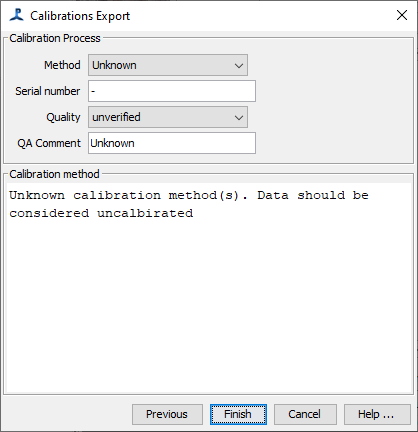
\includegraphics[width=0.98\linewidth,height=\textheight,keepaspectratio]{./media/cal2.png}

}

\subcaption{\label{fig-cal2}Calibration process details}

\end{minipage}%

\caption{\label{fig-cal}Calibration information dialog}

\end{figure}%

\begin{tcolorbox}[enhanced jigsaw, titlerule=0mm, rightrule=.15mm, opacitybacktitle=0.6, breakable, colframe=quarto-callout-tip-color-frame, coltitle=black, toptitle=1mm, bottomtitle=1mm, colback=white, title=\textcolor{quarto-callout-tip-color}{\faLightbulb}\hspace{0.5em}{See what you've exported so far}, arc=.35mm, bottomrule=.15mm, left=2mm, leftrule=.75mm, toprule=.15mm, colbacktitle=quarto-callout-tip-color!10!white, opacityback=0]

If you want to, at this point, skip to Section~\ref{sec-viewing} below
and look at what you've exported to Tethys using either the Tethys
Client or the internal PAMGuard tools.

\end{tcolorbox}

\subsection{Export the Deployments}\label{export-the-deployments}

Here, you'll get a chance to review the project information that you
entered earlier. This is critical information since any future analysis
will probably want to know the motivations behind the data collection.
For example were instruments laid out at random as part of a density
estimation study, or were you targeting an area known as a whale hotspot
anyway, in order to maximise detections for some other purpose.

Data Locations: This will default to the folders on your computer that
currently hold the sound files, the database and the binary store. If
you can, change these to where permanent copes of the data are stored,
e.g.~the server address or doi for the raw audio files you've used as in
Figure~\ref{fig-exportlocs}, (or perhaps for your data it's the name of
a cupboard full of hard drives in a dusty basemanet?). People may want
to find these data long after the computer you're currently using has
been recycled!

\begin{figure}

\begin{minipage}{0.50\linewidth}

\centering{

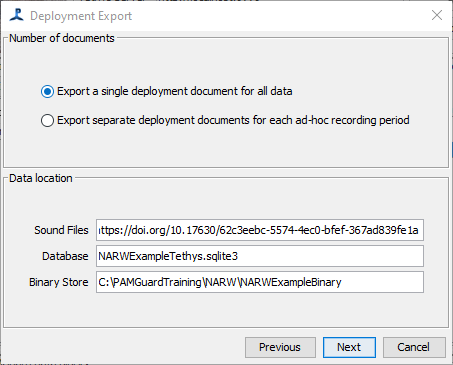
\includegraphics[width=0.98\linewidth,height=\textheight,keepaspectratio]{./media/exportlocs.png}

}

\subcaption{\label{fig-exportlocs}Data locations}

\end{minipage}%
%
\begin{minipage}{0.50\linewidth}

\centering{

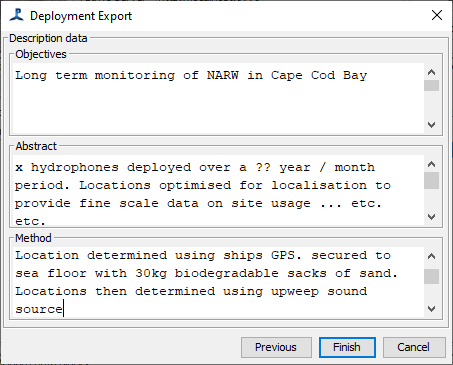
\includegraphics[width=0.98\linewidth,height=\textheight,keepaspectratio]{./media/deploymethod.png}

}

\subcaption{\label{fig-deploymethod}Deployment details entry}

\end{minipage}%

\caption{\label{fig-cal}PAMGuard dialogs for entering essential
information about the deployment. Tell people where to find the data,
which should ideally be an online archive rather than a folder on a
computer that may not exist in a years time. also say Where, why, and
how the data were collected. Knowing the motivation behind the data
collection is essential in understanding statistical models using those
data.}

\end{figure}%

\subsection{Export Detections and
Localizations}\label{export-detections-and-localizations}

\subsubsection{Species Codes}\label{species-codes}

PAMGuard will not allow you to export data to Tethys until you've
correctly defined species information for your detections.

Tethys uses ITIS Taxonomic Serial Numbers (TSN's) from the database at
\url{https://www.itis.gov/}. These are numeric codes for every known
species at all taxonomic levels, e.g.~you can have a code at the species
level (e.g.~180517 is for
\href{https://www.itis.gov/servlet/SingleRpt/SingleRpt?search_topic=TSN&search_value=180517\#null}{dens
beaked whale}), the Genus (180506 is for Mesoplodon), the Family (770799
is for Hyperoodontidae) all the way up to Animalia (202423). This is
important, since some detectors / classifiers really might be working at
the species level, for others you may just know that it's clicks or
whistles from an Odontocete (180404) but have no idea which species it
actually is.

Thinking of odontocetes raises another issue: Many odontocetes make
several types of call, for instance clicks, whistles, and burst pulse
sounds and you'll probably want to distinguish between them in your
database. Therefore, Tethys detections have both a compulsory ITIS
species code AND an optional call type.

Fortunately, you don't need to learn these species coded by heart or go
to the ITIS website to look them up (it's a bit slow) since they are all
already in the Tethys database you're working with and PAMGuard can
search for them.

In the lower left panel of the PAMGuard display, titled ``PAMGuard data
blocks'', right click on one of the rows in the table and select
``Species info'' to open the species code dialog.

Different PAMGuard detectors have different numbers of species defined.
For instance, the click detector has a `default' species that clicks
will be assigned to, which you'll probably set to Odontocete, but if
you're familiar with the click detector, you'll know that you can define
any number of species classifiers which may be for different
anthropogenic sounds as well as for different species of marine mammal.
For the DL classifier we're working with here, there are only two
classes: not right whales and right whales. The detector is designed to
only detect up-calls, so your species dialog should look similar to
Figure~\ref{fig-speciescodes}.

\begin{figure}

\centering{

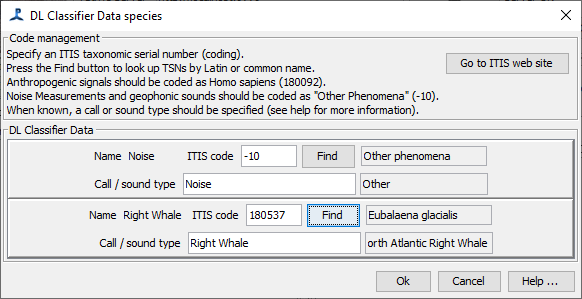
\includegraphics[width=0.7\linewidth,height=\textheight,keepaspectratio]{./media/speciescodes.png}

}

\caption{\label{fig-speciescodes}PAMGuard dialog for setting up ITIS
species codes. Some PAMGuard modules may only have a single species,
others, such as output from click and whistle classifiers may have many
set by the user. Each internal species name within PAMGuard must be
associated with an ITIS code}

\end{figure}%

Have a play around. Click on the `find button' and use the species
search dialog (Figure~\ref{fig-itis}) yourself. Try typing `right whale'
into the search term and you'll get a list of 13 different codes with
right whale in their name (I didn't expect that many either -- I though
there were three). Select the one you want and press OK.

\begin{figure}

\centering{

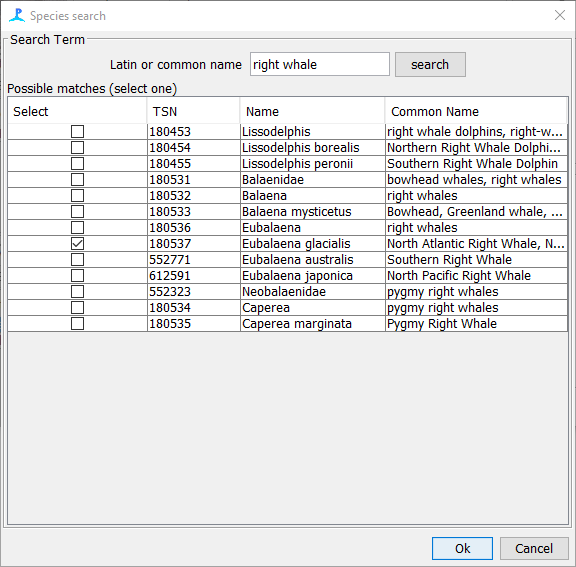
\includegraphics[width=0.6\linewidth,height=\textheight,keepaspectratio]{./media/itis.png}

}

\caption{\label{fig-itis}The PAMGuard ITIS Species code search dialog}

\end{figure}%

\begin{tcolorbox}[enhanced jigsaw, titlerule=0mm, rightrule=.15mm, opacitybacktitle=0.6, breakable, colframe=quarto-callout-note-color-frame, coltitle=black, toptitle=1mm, bottomtitle=1mm, colback=white, title=\textcolor{quarto-callout-note-color}{\faInfo}\hspace{0.5em}{Note}, arc=.35mm, bottomrule=.15mm, left=2mm, leftrule=.75mm, toprule=.15mm, colbacktitle=quarto-callout-note-color!10!white, opacityback=0]

Putting these codes into multiple similar projects can get a bit
tiresome. It's not possible to make a ``standard'' translation between
the codes that PAMGuard detector use and ITIS since everyone sets up
PAMGuard in a different way. However, I am thinking about ``Export'' and
``Import'' buttons on these dialogs so that you can move the TSN
translations between your own projects more efficiently.

\end{tcolorbox}

\subsubsection{Export the Data}\label{export-the-data}

\begin{figure}

\begin{minipage}{0.33\linewidth}

\centering{

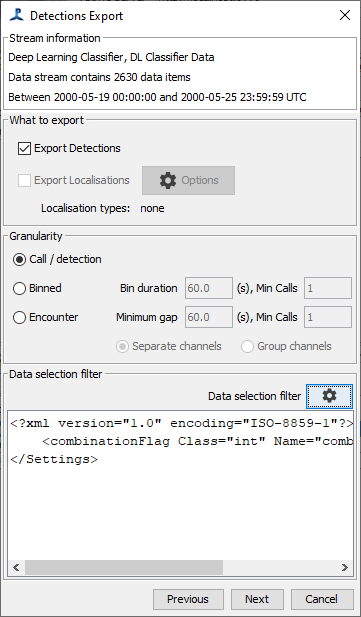
\includegraphics[width=0.99\linewidth,height=\textheight,keepaspectratio]{./media/export2.png}

}

\subcaption{\label{fig-export2}What to export}

\end{minipage}%
%
\begin{minipage}{0.33\linewidth}

\centering{

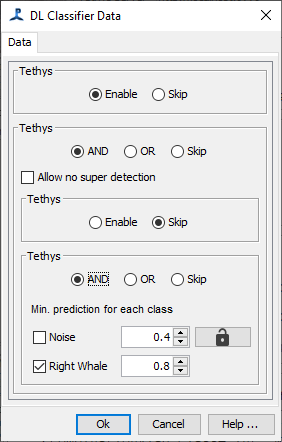
\includegraphics[width=0.99\linewidth,height=\textheight,keepaspectratio]{./media/dataselection.png}

}

\subcaption{\label{fig-datasel}Data Selection}

\end{minipage}%
%
\begin{minipage}{0.33\linewidth}

\centering{

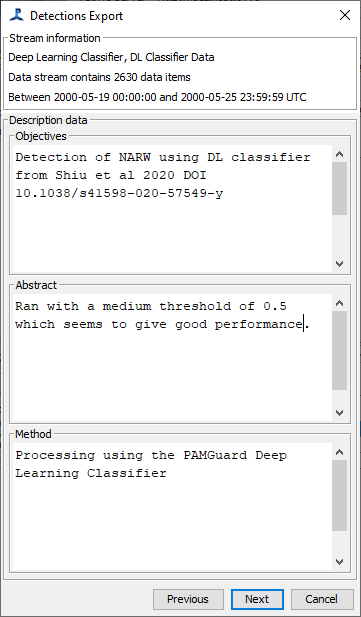
\includegraphics[width=0.99\linewidth,height=\textheight,keepaspectratio]{./media/export3.png}

}

\subcaption{\label{fig-export3}Details about the data}

\end{minipage}%
\newline
\begin{minipage}{0.33\linewidth}

\centering{

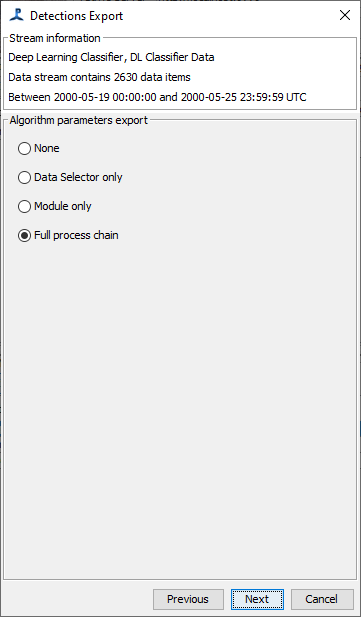
\includegraphics[width=0.99\linewidth,height=\textheight,keepaspectratio]{./media/export4.png}

}

\subcaption{\label{fig-export4}Algorithm parameters}

\end{minipage}%
%
\begin{minipage}{0.33\linewidth}

\centering{

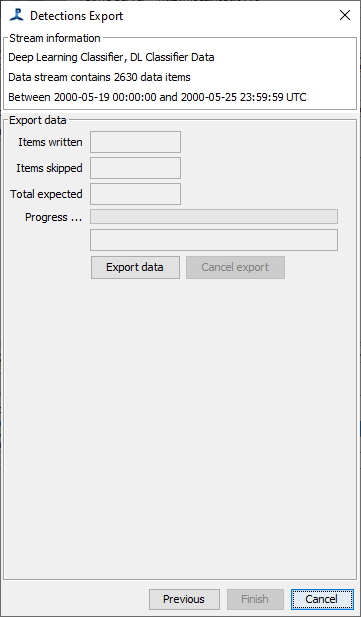
\includegraphics[width=0.99\linewidth,height=\textheight,keepaspectratio]{./media/export5.png}

}

\subcaption{\label{fig-export5}Export progress}

\end{minipage}%

\caption{\label{fig-export}Pages of the Detection and Localization
export wizard.}

\end{figure}%

Once the species codes are all in place, you can export the detections
by pressing the ``Export \ldots{}'' button.

Again, this will take you through several pages of a ``Wizard'', as
shown in Figure~\ref{fig-export} where you'll enter more information.
The first page is filled in automatically with information about the
detector and the PAMGuard version you're running.

The second page, Figure~\ref{fig-export2} is much more interesting,
where you'll chose whether you export Detections, Localizations, or
both. If you're doing both, it's a good idea to do them at the same time
so that the Localizations document can easily cross reference to the
Detections. Note that these data don't have any localizations, so that
options is not available. You'll also select the \textbf{Granularity}
which can be ``Call'', ``Binned'', or ``Encounter''.

\textbf{``Call''}: If you select call, then every single call in your
dataset will be exported to Tethys. This is probably OK for baleen
whales, where data rates are not too low, but we'd advise against trying
to export too many millions of clicks from an odontocete dataset.

\textbf{``Binned''}: This exports counts of data in fixed time intervals
of your choosing which could be seconds or days. If you like C-POD
porpoise positive minutes, this is the option for you. For data with a
high call rate it's certainly a good way of getting a summary of your
detections into Tethys without overloading it. Note that if more than
one species (see the species codes section above) is present within a
time interval, then an entry will be made in the database for each
different species.

\textbf{``Encounter''}: This option searches for groups of sounds close
together in time and saves a record with the start and end time of the
encounter along with a count of the number of calls within that time
period.

For Binned and Encounter export you can also choose to separate
individual channels. This might make sense if your hydrophones are
spatially very far apart so that you're getting different animals
detected on each one. It's your data and it's up to you.

\textbf{Data Selection filters}

Some PAMGuard outputs (not all) have a data selection filter for the
deep learning classifier. These are used by multiple PAMGuard components
and are generally quite bespoke for each detector. For example, the Deep
Learning data selector (Figure~\ref{fig-datasel}) has been set to only
export data with a score of 0.8 or more, which is a subset of the data
since the detector was set to save detections with a score of 0.4 or

The data selector in click detector allows you to select by click type
(if you're using click classifier) and whether clicks are assigned to a
click train. The click data selector is used on various displays and
also to filter input to the click train detector. The right whale edge
detector allows you to select by the `score' of the detection. The DL
right whale detector does not yet have a data selector, but I may add
one, whereby you can also select by score. If there is a data selector,
then information about it will be shown at the bottom of the granularity
page.

\textbf{Detections information} (more abstracts and stuff)
Figure~\ref{fig-export3}

This again ? Didn't you enter this for the Deployment document you
created ? Yes, but it's important since the motivations behind your
analysis have to be captured separately from the motivations behind the
overall study. For example, the deployment may have been to survey all
baleen whale species over a period of months, but the analysis may have
only concentrated on a single species. Think about what someone trying
to use these data after you've retired or moved to another job may need
to know and enter it here.

\textbf{Algorithm Parameters} Figure~\ref{fig-export4}

Here you can capture all the information about the processing that took
place in PAMGuard. It will be written to the top of each Detections
document in xml format. The options are reasonably self explanatory: for
instance for the right whale edge detector, if you select `Full Process
Chain', you'll get all of the settings not just of the detector, but the
FFT module feeding it, and the acquisition module feeding the FFT (and a
decimator or any other modules upstream of the detector). The easiest
way to understand this is to generate some outputs and take a look at
what's in the XML. Generally, we'd recommend outputting the ``Full
Process Chain''. It's a bit verbose, but does give a complete record of
how PAMGuard was set up for processing the data -- which is one of the
key goals of Tethys.

\textbf{Export the Data} Figure~\ref{fig-export5}

The last page of the Wizard has the ``Export data'' button, which will
generate the Tethys records and write them to the database.

\emph{Large datasets}

Exporting very large datasets can take a very long time and may even
bring down the system with memory overflows. We're still working on how
to manage this and any feedback will be welcome.

You should experiment with exporting data in different ways: Try the
different granularities and see what you get. See what difference there
is in the data recorded from two detectors.

\section{Viewing and Managing the Data}\label{sec-viewing}

\subsection{The Tethys Web Client}\label{the-tethys-web-client}

By far the most versatile way to view data is to use the Web based
client developed by Marie Roch. You'll have seen instructions on how to
launch this with the Tethys installation instructions. To make life
easy, instead of typing `localhost:9779/Client' into your web browser,
you can just hit the `Open Client' button at the top of the display.

\subsection{List of Documents}\label{list-of-documents}

To the right of the `Open Client' button, there is a small drop down
arrow. This will show a menu that takes you to lists of Tethys documents
(all documents of a particular type in the database) which can be either
in the web browser, or within PAMGuard. Try both, using the `Show in
PAMGuard' option to switch between browser view and PAMGuard view.

\subsection{View a Single Document}\label{view-a-single-document}

To check the output of a single document, the easiest thing to do is to
simply right click on it in the PAMGuard display and select `Display
document \ldots{}' and a window will appear with the XML text of the
document.

\subsubsection{Deleting Data}\label{deleting-data}

We all make mistakes (Well, I do!). The displays in PAMGuard will
generally show a pop-up menu with a delete option which will remove any
documents from the database.

\subsection{Exporting}\label{exporting}

Similarly, there is an option to save individual documents as XML text
documents.

\section{When things go wrong}\label{when-things-go-wrong}

This is new software, hot out of the mines, so expect a few teething
problems. We really value feedback and information on errors since
that's the only way we can rectify problems. If there is an error
writing a document, you should get a big clear pop-up window saying that
the document failed to write. In the corner of that window is a `Copy'
button which will copy the text of the error into the systems clipboard.
Please do that and paste it into an email to us at
\href{mailto:info@pamguard.org}{\nolinkurl{info@pamguard.org}}.

Another really helpful thing you can do at this point is to also get a
copy of the XML document that PAMGuard was attempting to write to the
Tethys database. Prior to writing to the database, these are held in a
temporary folder and they are deleted when you exit PAMGuard. The folder
can be tricky to find (on my system it's in
C:\textbackslash Users\textbackslash dg50\textbackslash Pamguard\textbackslash PAMGuardTethys)
but there is a menu item `open temp document folder' at the bottom of
the documents menu (the one next to the `Open client' button) and also
in the Settings / Tethys menu. If you can attach a copy of the document
that caused an error to an email to us, then we'll be able to fix it.
Finally, if you've not found it before, PAMGuard logs the terminal
output in a set of files in the user/Pamguard folder (mine is
C:\textbackslash Users\textbackslash dg50\textbackslash Pamguard). You
can get to this from the main PAMGuard help menu. The files may look as
though they are full of total garbage, but it's meaningful to us and can
help us to debug any problems effectively and efficiently.

\section{What's Next ?}\label{whats-next}

There are a couple of things that we've not yet included in the PAMGuard
Tethys interface.

\subsection{Localisation Data}\label{localisation-data}

Tethys stores Localisations separately to Detections. We've spent a lot
of time in recent weeks discussing exactly what to store for each type
of localisation and are ready to start programming this into both Tethys
and PAMGuard. For the user, the export of Localisations will look very
similar to that of Detections (and may even be integrated into the same
export dialog). Anyone interested in discussing this should do so during
the meeting. Test datasets to develop code on are always welcome!

\subsection{Track Survey Effort}\label{track-survey-effort}

PAMGuard has never had a great way of handling trackline data. Yes, it's
good at storing GPS data, but doesn't have any infrastructure to say
``This bit of track is transect number 1'', ``This bit is off-effort'',
etc. Several users have come up with ad-hoc solutions to this problem,
for instance using the PAMGuard Logger Forms, or even running the old
Logger software in parallel. We'll be developing methods to try to
standardise this in PAMGuard and welcome example datasets or comments on
how you might like to do this.

\subsection{Annotation Effort}\label{annotation-effort}

A critical component of the Detections documents is the ``Effort'' that
went into creating the detections. For the automatic detectors,
gathering this information is easy, since the times that the detectors
ran is already in the PAMGuard dataset. However, PAMGuard also allows
for human annotation in several of its modules which includes the
assignment of clicks to click trains and marking out sounds on the
spectrogram. If you've used it carefully, there is an annotation effort
module in PAMGuard, but a) that's quite new so a lot of data have been
annotated without it and b) humans are human and don't always fill in
the correct fields when they start work. Finding a system where we can
correctly record annotation effort for the different detectors is
another thing we're working on and will incorporate into future
releases.

\section{References}\label{references}

\phantomsection\label{refs}
\begin{CSLReferences}{1}{0}
\bibitem[\citeproctext]{ref-gillespie2004}
Gillespie, D. 2004. {``Detection and Classification of Right Whale Calls
Using an Edge Detector Operating on a Smoothed Spectrogram.''}
\emph{Canadian Acoustics} 32: 39--47.
\url{https://jcaa.caa-aca.ca/index.php/jcaa/article/view/1586}.

\bibitem[\citeproctext]{ref-roch2016}
Roch, Marie A., Heidi Batchelor, Simone Baumann-Pickering, Catherine L.
Berchok, Danielle Cholewiak, Ei Fujioka, Ellen C. Garland, Sean Herbert,
John A. Hildebrand, and Erin M. Oleson. 2016. {``Management of Acoustic
Metadata for Bioacoustics.''} \emph{Ecological Informatics} 31: 122136.
\url{https://doi.org/doi.org/10.1016/j.ecoinf.2015.12.002}.

\bibitem[\citeproctext]{ref-shiu2020}
Shiu, Yu, K. J. Palmer, Marie A. Roch, Erica Fleishman, Xiaobai Liu,
Eva-Marie Nosal, Tyler Helble, Danielle Cholewiak, Douglas Gillespie,
and Holger Klinck. 2020. {``Deep Neural Networks for Automated Detection
of Marine Mammal Species.''} \emph{Scientific Reports} 10 (1).
\url{https://doi.org/10.1038/s41598-020-57549-y}.

\end{CSLReferences}




\end{document}
